\documentclass[runningheads,a4paper]{llncs}

\usepackage{amssymb}
\setcounter{tocdepth}{3}
\usepackage{graphicx}

\usepackage{url}
\urldef{\mailsa}\path|{dschenkelman, mservetto}@fi.uba.ar|
\newcommand{\keywords}[1]{\par\addvspace\baselineskip
\noindent\keywordname\enspace\ignorespaces#1}

\begin{document}

\mainmatter  % start of an individual contribution

% first the title is needed
\title{Using algorithmic skeletons in EcmaScript to parallelize computation in browsers through Web Workers}

% a short form should be given in case it is too long for the running head
\titlerunning{Algorithmic skeletons to parallelize computation in browsers}

% the name(s) of the author(s) follow(s) next
%
% NB: Chinese authors should write their first names(s) in front of
% their surnames. This ensures that the names appear correctly in
% the running heads and the author index.
%
\author{Damian Schenkelman\and Matias Servetto}
%
\authorrunning{Algorithmic skeletons to parallelizing computation in browsers}
% (feature abused for this document to repeat the title also on left hand pages)

% the affiliations are given next; don't give your e-mail address
% unless you accept that it will be published
\institute{School of Engineering. University of Buenos Aires.\\
Paseo Colon 850, Buenos Aires, Argentina\\
\mailsa\\
\url{http://www.fi.uba.ar/}}

%
% NB: a more complex sample for affiliations and the mapping to the
% corresponding authors can be found in the file "llncs.dem"
% (search for the string "\mainmatter" where a contribution starts).
% "llncs.dem" accompanies the document class "llncs.cls".
%

\toctitle{Lecture Notes in Computer Science}
\tocauthor{Authors' Instructions}
\maketitle


\begin{abstract}
With the growing tendency of browsers being used for CPU intensive applications (such as 3D games) it is important to take advantage of multiple cores to reduce user perceived latency. This paper presents a JavaScript library based on algorithmic skeletons that allows users to take advantage of parallel processing in browsers while maintaining a familiar coding style.
\keywords{browsers, ecmascript, parallelization, algorithmic skeletons}
\end{abstract}

\section{Introduction}

In 1965 Gordon Moore proposed the popularly known ``Moore's law" \cite{moore65}, which predicts that the number of transitors in integrated circuits will double every two years.
As a consequence, programs that use a single processor/core will automatically become faster without the need to modify them with that purpose in mind.

In the year 2010 it was predicted that this tendency would be slowly reaching its end, mostly due to reasons related to heat dissipation. This is the reason why newer computers have a greater number of processors instead of processors with more computing power.

To be able to maximize the performance of these computers, it is paramount that systems professionals can create programs that process data in parallel, through different mechanisms, such as threads or processes executing simultaneously in different processors. In the case of applications executed on a single device (e.g. browsers and web pages, applications for mobile devices, desktop apps, server applications) a lot of languages and platforms provide a simple way for programmers to abstract the complexity and coordination required for this type of processing. For example, the .NET platform has the Task Parallel Library (TPL) and Parallel LINQ (PLINQ) \cite{ms-par} libraries that use algorithmic skeletons modelled with high order functions so developers can perform complex operations through a simple API.

On a different note, one of the tendencies that is beginning to take off is the use of EcmaScript \cite{es-web} (also known as Javascript) to create applications, such as video games, that were previously only considered viable in a native environment. This has been possible thanks to components like asm.js \cite{asm-web} and WebGL \cite{webgl-web} together with the constant evolution of browsers and JavaScript runtime engines.
In this context, one of the plans of the commitee that develops the language is to provide an API to simplify the processing of data in parallel for version 7 (ES7) of the language, with the goal of keeping up with native applications. Initiatives such as ParallelJS \cite{par-js} and River trail \cite{rivertrail} or the possibility of taking advantage of SIMD instructions \cite{js-simd} (single instruction multiple data) are some of the options to implement this.

The goal of this paper is to provide an alternative for parallel code execution in EcmaScript, through a library that exposes high order functions to model algorithmic skeletons such as map, filter and reduce. This library will take advantage of Web Workers \cite{w3c-ww} (the mechanism proposed by browsers for parallelism at the time of writing) to allow the simultaneous execution of code in multiple processors.

This paper is organized as follows: Section~\ref{sec:background} provides some context on the current state of thread-base parallelization in JavaScript. Section~\ref{sec:overview} provides an overview of how the library works. Section~\ref{sec:implementation} explains the challenges the library faces, the alternative solutions and the decisions taken. Section~\ref{sec:experiment} compares the performance of using the library against a sequential approach for an image transformation. Finally, Section~\ref{sec:future} presents future research directions.

\section{Background}\label{sec:background}
All modern versions of major browsers (Internet Explorer, Mozilla Firefox, Google Chrome, Safari and Opera) allow the execution of JavaScript code in a single threaded event loop runtime \cite{event-loop}. User actions add elements to the event loop queue and these are processesed sequentially. All process input/output is asynchronous to prevent the UI thread from blocking, thus keeping it responsive.
While such a runtime is a good fit for most web applications, JavaScript and the browser are now also being used for some CPU intensive tasks, such as games, which commonly require physics calculations, image manipulation (in 2D) and graphics generation (in 3D). Despite the large improvement in JavaScript's performance, obtained through optimizing compilers such as Google Chrome's V8 \cite{v8} and Mozilla Firefox's SpiderMonkey \cite{spider-monkey}, it is important to be able to take advantage of multiple cores in modern devices to achieve even greater performance.\\
In 2010, Web Workers were made part of the web standard. Web Workers allow the creation of ``thread like'' constructs in a browser environment, but they don't allow shared memory and instead communicate via message passing. The message passing overhead is very big for common objects and Web Workers ``have a high start-up performance cost'' \cite{w3c-ww}, so they were commonly considered for long running tasks and operating on generally the same set of data during a single execution, making them unfit for a thread pool  model \cite{thread-pool}.\\
However, a spec is being developed for version 7 of the EcmaScript standard that changes this, by introducing shared memory through \verb+SharedArrayBuffer+s \cite{sab}. In essence, the proposal allows the same memory to be shared across multiple Web Workers, and also aims to provide the necessary atomic/lock constructs to deal with shared memory. In the particular case of embarrassingly parallel computations (such as map, filter and reduce operations on an array), it is simple to take advantage of the speed benefits of shared memory without incurring in any overhead due to synchronization.

\section{Library Overview}\label{sec:overview}
JavaScript developers are familiar with the concept of map, filter and reduce skeletons as language constructs. In JavaScript, \verb+Array+s have \verb+map+, \verb+filter+, and \verb+reduce+ functions and version 6 of the EcmaScript standard adds those same methods to \verb+TypedArray+s \cite{es6-ta}. For example, to multiply all the elements of an \verb+Array+ by two:
\medskip

\noindent
{\it plain JS map sample}
\begin{verbatim}
var newValues = [1,2,3,4].map(function(e){
  return e * 2;
});

// newValues is a new array [2,4,6,8]
\end{verbatim}
%
\noindent
{\small (Example creating a new array with the values of the original one multiplied by two)}\\

Our library (p-j-s) only works with \verb+SharedTypedArray+s (and \verb+TypedArray+s) due to performance reasons discussed in Section~\ref{sec:implementation}. It aims to provide a similar interface while not changing the native object's prototypes and dealing with the asynchronous nature of the operation. Given a \verb+SharedTypedArray+, the following code would do the same as the previous example but parallelizing the work:
\medskip

\noindent
{\it p-j-s map sample}
\begin{verbatim}
var pjs = require('p-j-s');
pjs.init({ maxWorkers: 4 });
var xs = new SharedUint8Array(4);
xs.set([1,2,3,4]);
pjs(xs).map(function(e){
  return e * 2;
}).seq().then(function(newValues){
  // newValues is a new SharedUint8Array [2,4,6,8]
});
\end{verbatim}
%
\noindent
{\small (Example creating a new array with the values of the original one multiplied by two using p-j-s)}\\

The call to \verb+pjs.init+ initializes the library and the amount of workers to be used for processing (a worker pool is created with them). In browsers that have an API to detect the amount of available cores in a machine, the \verb+maxWorkers+ value is limited by the amount of cores.

The API provided by p-j-s \cite{pjs-api} is very similar to the synchronous one that is provided by the language. The asynchronous nature of the operation is reflected by the fact that the call to \verb+seq+ returns a \verb+Promise+ \cite{promise} (alternatively a callback could be passed as a parameter to it).

It is possible to chain multiple operations before calling \verb+seq+ to avoid passing data back and forth between the Web Workers and the UI thread. Before \verb+seq+ is invoked, an operation is a chain of one or more steps. From the same main chain, multiple chains could be created:
\medskip

\noindent
{\it p-j-s chaining sample}
\begin{verbatim}
var xs = new SharedUint8Array(4);
xs.set([1,2,3,4]);

var chain = pjs(xs).map(function(e){
  return e * 3;
});

var evenChain = chain.filter(function(e){
  return e % 2 === 0;
});

var sumChain = chain.reduce(function(c, v){
  return c + v;
}, 0, 0);

evenChain.seq().then(function(evens){
  // evens is [6, 12]
  sumChain.seq().then(function(sum){
    // sum is [3,6,9,12]
  });
});
\end{verbatim}
%
\noindent
{\small (Example creating multiple chains from the same base chain)}\\

\section{Implementation}\label{sec:implementation}
Let's consider an array of \verb+N+ elements on which a particular transformation is to be performed through the \verb+map+ function. If the transformation is executed using a single thread (no parallelism) and the average time to process each element is \verb+t+ then the total time (\(T_{ser}\)) for the operation can be approximated as:

\begin{equation}
  T_{ser} = \sum_{i = 0}^{N}t = Nt \;  .
\end{equation}

When trying to parallelize this operation using \(K\) threads the ideal goal is to reach a total time (\(T_{par}\)) that is:

\begin{equation}
  T_{par} = \frac{T_{ser}}{K} \;  .
\end{equation}

Nevertheless, there are additional time consuming tasks other than the main computation that need to be considered when performing the operation in parallel in programs where not all memory is shared. These are:
\begin{itemize}
  \item Serializing/deserializing the elements to transfer.
  \item Transferring the elements back and forth between the UI thread and the workers.
  \item Serializing/deserializing the function to transfer.
  \item Transferring to each worker the functions for the transformation.
\end{itemize}

If we drill down into the different parts:
\begin{itemize}
  \item \(T_{ft}\) as the function transfer time
  \item \(T_{et}\) as the elements transfer time
  \item \(T_{fs}\) as the function serialization/deserialization time
  \item \(T_{es}\) as the elements serialization/deserialization time
\end{itemize}

It is clear that:
\begin{equation}
  T_{sync} = T_{ft} + T_{et} + T_{fs} + T_{es} \;  .
  \label{eq:tsync}
\end{equation}

\begin{equation}
  T_{par} \approx \frac{T_{ser}}{K} + T_{sync} \;  .
  \label{eq:tpar}
\end{equation}

Based on Eq.~\ref{eq:tsync} and Eq.~\ref{eq:tpar} it can be deduced that the more \(T_{sync}\) can be reduced, the closer to the ideal scenario the computation will be.

In our case we are trying to transfer objects between a browser's JavaScript UI thread and Web Workers so we are constrained by the means of that environment. The Worker interface is the following \cite{w3c-ww}:
\medskip

\noindent
{\it Web Worker interface}
\begin{verbatim}
[Constructor(DOMString scriptURL)]
interface Worker : EventTarget {
  void terminate();

  void postMessage(any message, optional sequence<Transferable> transfer);
  [TreatNonCallableAsNull] attribute Function? onmessage;
};
Worker implements AbstractWorker;
\end{verbatim}
%
\noindent
{\small (Example extracted from the W3C Web Workers specification)}

As the aforementioned interface states one can either send just a message or send a message with a sequence of transferable objects. From section \textbf{2.7.5} of the HTML Standard \cite{html-whatwg}:
\textit{``Some objects support being copied and closed in one operation. This is called transferring the object, and is used in particular to transfer ownership of unsharable or expensive resources across worker boundaries."}

\subsection{Elements}
Considering the definition of a \verb+Transferable+, it seems like a good alternative to minimize both \(T_{et}\) and \(T_{es}\). Even more so when one considers that otherwise objects are copied using structured cloning (explained in section \textbf{2.7.6} of that same standard).

To verify our hypothesis, we put together two benchmarks\footnote{All benchmarks in this document use the environment described in Tab.~\ref{tab:env}.} that aim to verify the difference between invoking \verb+postMessage+ with and without structured cloning for a \verb+SharedTypedArray+. Both transfer a \verb+SharedTypedArray+ back and forth between the UI thread and a worker; the only difference between the two is that one\footnote{http://jsperf.com/transferrable-vs-cloning/2} has 100,000 (a hundred thousand) elements in the \verb+SharedTypedArray+ and the other one\footnote{http://jsperf.com/longer-transferrable-vs-cloning/2} 1,000,000 (a million). As it can be seen from the  results in Tab.~\ref{tab:transf-vs-clone}, increasing the amount of elements by 10x does not change the amount of operations that can be performed when using \verb+Transferable+ objects; it scales. On the other hand, the amount of operations that can be performed with structured cloning greatly decreases. For that reason our library only works with \verb+SharedTypedArray+s and \verb+TypedArrays+.

\begin{table}
  \centering
  \begin{tabular}{|l|l|}
    \hline
    Computer & Mac Book Air \\
    Processor & Intel Core i5 \\
    Clock Frequency & 1.8 GHz \\
    System Memory & 4 GB \\
    Operating System & OS X Yosemite 10.10.3 \\
    Browser version & Firefox Nightly 41.0a1 \\
    \hline
  \end{tabular}
  \caption{Benchmarks environment.}
  \label{tab:env}
\end{table}

\begin{table}
  \centering
  \begin{tabular}{|c|c|c|}
    \hline
    Elements & Cloning [ops/sec] & Transferring [ops/sec] \\
    \hline
    \(1E5\) & 734 & \textbf{1596} \\
    \(1E6\) & 91 & \textbf{1134} \\
    \hline
  \end{tabular}
  \caption{Difference between transferring and cloning shared buffers.}
  \label{tab:transf-vs-clone}
\end{table}

\subsection{Functions}\label{sub-sec:functions}
The library must handle the distribution of the code between the different workers when an operation is executed. This is a challenging problem with many possible alternatives: Cloud Haskell \cite{cloud-haskell} for example, requires a customized version of the Glasgow Haskell Compiler (GHC) to serialize closures and their captured variables as a code pointer and an environment, operating under the assumption that the same code is executed in all nodes. A proposal for using Scheme for distributed programming \cite{distributed-scheme} uses a custom serializable data structure to represent procedures, and macros in order to capture a closure's captured variables and serialize their values. It also assumes that all nodes are executing the same program since serialized functions store pointers to parts of source code files.

In our case, modifying the runtime is not a viable alternative since we want our library to be usable by anyone creating applications for major browser versions.

A naive approach would be to try to transfer a function as part of the \verb+message+ parameter of \verb+postMessage+ but that is not an option (it throws an error).

Considering the fact that \verb+Function+ objects cannot be directly transferred a different serialization approach is to be considered a possible alternative is to:
\begin{enumerate}
  \item Serialize the \verb+Function+ to a \verb+String+.
  \item Transfer the \verb+String+ to the worker.
  \item Create a new \verb+Function+ on the worker from that \verb+String+.
\end{enumerate}

Sec.~\ref{sub-sec:context} proposes a solution to sharing additional data and functions between the UI thread and Web Workers as a replacement for variables captured by closures.

\subsubsection{Serialization and deserialization}
One possible way of passing serialized \verb+Function+ to workers would be to encode them as binary and transfer them as an \verb+ArrayBuffer+. To encode the strings there are two possible approaches:
\begin{itemize}
  \item Using the Encoding API\cite{encoding-api}
  \item Implementing non native encoding/decoding functions
\end{itemize}

The results for the benchmark\footnote{http://jsperf.com/pjs-serialization-comparison/2} are in Tab.~\ref{tab:encode-decode}:
\begin{table}
  \centering
  \begin{tabular}{|c|c|}
    \hline
    Native encoding API [ops/sec] & Non-native function [ops/sec] \\
    \hline
    \textbf{5017} & 4398 \\
    \hline
  \end{tabular}
  \caption{Difference encoding/decoding strings natively and in JavaScript.}
  \label{tab:encode-decode}
\end{table}

\subsubsection{Transference}
\verb+Function+'s code not only needs to be serialized but also transferred. For that reason it was also worth comparing the time it takes to encode/decode a \verb+String+ and tranfer the resulting \verb+ArrayBuffer+ to the worker against just passing the \verb+String+ to the worker.

Additionally, in most scenarios code would have to be sent along with a \verb+TypedArray+ so it would also be interesting to see if the transfer time was affected by this fact.

We created benchmarks\footnote{http://jsperf.com/pjs-serialization-long/3 and http://jsperf.com/pjs-serialization/3} using two functions whose string representation has different lengths to see if the function's length affected the serialization and transfer time (results in Tab.~\ref{tab:send-function}). We measured three approaches to transfer the string:
\begin{enumerate}
  \item Encoding the \verb+String+ into an \verb+TypedArray+, sending it as a \verb+Tranferable+ and decoding it on the Web Worker.
  \item Sending the \verb+String+ directly.
  \item Using a \verb+Blob+ to store the stream and retrieving that in the Worker.
\end{enumerate}

\begin{table}
  \centering
  \begin{tabular}{|c|c|c|c|}
    \hline
    Function length & Blob [ops/sec] & Copy [ops/sec] & Tranferable [ops/sec] \\
    \hline
    Short & 1070 & \textbf{6629} & 5927 \\
    Long & 1075 & \textbf{3273} & 2967 \\
    \hline
  \end{tabular}
  \caption{Sending function strings from UI thread to Web Workers.}
  \label{tab:send-function}
\end{table}

We created a separate benchmark\footnote{http://jsperf.com/shared-function-transfer} to compare the best option (copying) against encoding the function into a \verb+SharedTypedArray+ and transferring it to four workers. We expected the latter to be slower since it involves encoding the code once and decoding it in each worker. The results are shown in Tab.~\ref{tab:copy-vs-shared}.

\begin{table}
  \centering
  \begin{tabular}{|c|c|}
    \hline
    Copying [ops/sec] & SharedArrayBuffer [ops/sec] \\
    \hline
    \textbf{1315} & 1226 \\
    \hline
  \end{tabular}
  \caption{Sending code to four workers by copying compared to encoding it and using a SharedArrayBuffer.}
  \label{tab:copy-vs-shared}
\end{table}

We also created a benchmark\footnote{http://jsperf.com/pjs-encoding/2} that tranfers a \verb+SharedTypedArray+ and a \verb+String+ that are properties of the same \verb+message+ object back and forth between the UI thread an a Web Worker to understand if transferring additional objects affected the transfer time when comparing it with just tranferring a \verb+String+ (results in Tab.~\ref{tab:send-function-and-array}).
\begin{table}
  \centering
  \begin{tabular}{|c|c|}
    \hline
    Copying code [ops/sec] & Tranferring code [ops/sec] \\
    \hline
    \textbf{4509} & 4270 \\
    \hline
  \end{tabular}
  \caption{Sending code and a TypedArray to a Web Worker.}
  \label{tab:send-function-and-array}
\end{table}

\subsection{Contexts}\label{sub-sec:context}
Functions in JavaScript can capture variables as long as they are within the variable's lexical scope. Functions that make use  of this feature are closures. As explained in subsection~\ref{sub-sec:functions}, \verb+Function+ objects cannot be passed as messages to workers. This means that there is no out of the box mechanism to make variables that are available in the environment when the parallel computation is started accessible when executing the callback functions in each Web Worker.

To solve this problem, p-j-s introduces the \emph{context} concept. There are two kinds of contexts:
\begin{description}
\item[Global context] Shared across all chains.
\item[Local context] Specific to a particular step in a chain.
\end{description}

The following code snippet shows how developers can work with each type of context:
\medskip

\noindent
{\it p-j-s context sample}
\begin{verbatim}
var xs = new SharedUint8Array(4);
xs.set([1,2,3,4]);

pjs.updateContext({
  max: 3
}).then(function(){
  pjs(xs).filter(function(e, ctx){
    return e <= ctx.max && e >= ctx.min;
  }, {
    min: 2
  }).seq().then(function(range){
    // range is [2,3]
  });
});

\end{verbatim}
%
\noindent
{\small (Example using local and global context for chains)}\\

When executing each step in a chain, the local context is merged with the global context (neither is modified) into a separate object which is the \verb+ctx+ parameter that the function receives. If the same key is present in both the global and local context, the one in the local context is the one that will be available. Given the following code snippet, the available \verb+ctx+ for each function is displayed in Fig.~\ref{fig:context}.
\medskip

\noindent
{\it p-j-s context merge sample}
\begin{verbatim}
var xs = new SharedUint8Array(4);
xs.set([1,2,3,4]);

pjs.updateContext({
  A: 0,
  B: 25,
  C: 44
}).then(function(){
  var chain = pjs(xs)
    .map(function(e, ctx){
      // code here
    }, { A: 5, B: 13 })
    .filter(function(e, ctx){
      // code here
    }, { A: 2, E: 9 })
});

\end{verbatim}
%
\noindent
{\small (Example for resulting ctx)}\\

\begin{figure}
\centering
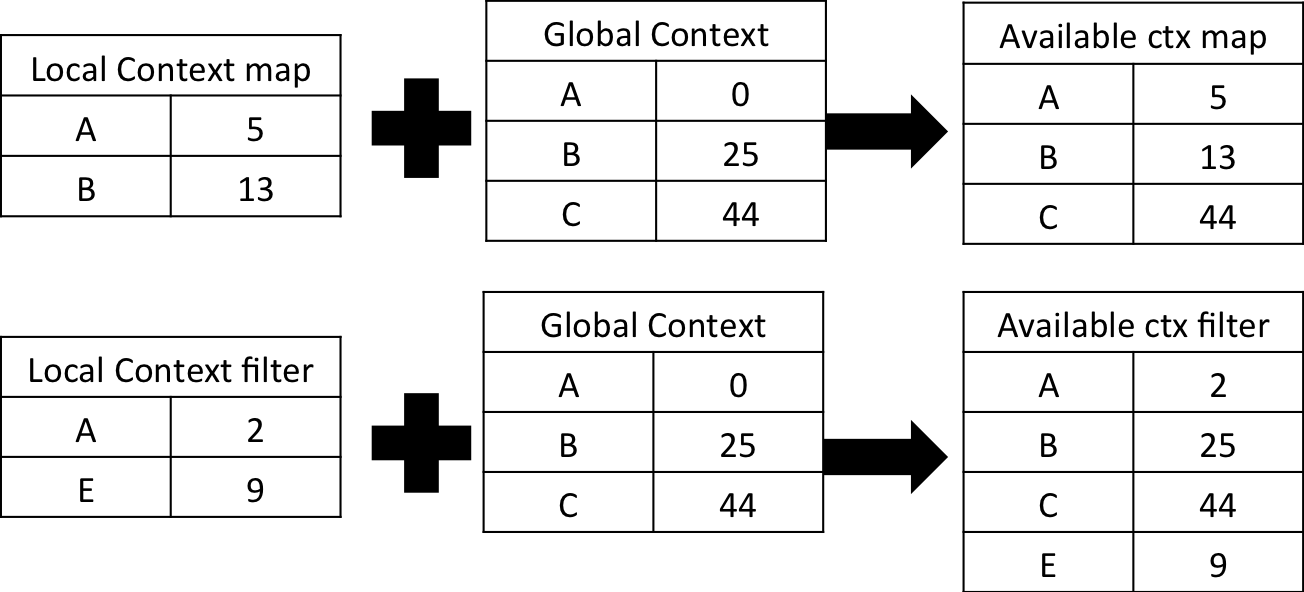
\includegraphics[width=1\textwidth]{context}
\caption{Example of global and local context being merged for chain steps.}
\label{fig:context}
\end{figure}

One alternative to hide the \emph{context} concept from application developers could be to introduce a \textit{build} step that detects the variables captured by p-j-s callbacks and transforms the code. By doing this, they wouldn't need to do anything out of the ordinary with regards to closures and their environment when working with p-j-s. However, this approach would require transforming the original code, and would be complex and time consuming to implement.

\section{Experiment}\label{sec:experiment}
It is important to compare the performance of our parallel implementation against a serial one, as some processing is required before the computation begins and after it ends to distribute the data and work and gather the results respectively, as explained in Section~\ref{sec:implementation}.

In this regard, the more complex the computation to be performed on each array element the better the parallel implementation will perform. The reason for this is that, in the parallel case, the cost of this processing is dwarfed by the cost of the actual computation.

\subsection{Algorithm selection}
For the experiment we decided to use an algorithm that applies a sepia tone effect to pictures. This meets the criteria of both being useful and having some calls to \verb+Math.random+ which make it more complex from a computational standpoint. The benchmark is publicly available \cite{benchmark}.

\subsection{Results}
The results for the benchmark are the displayed in Tab.~\ref{tab:benchmark}. Based on those results, we created a chart (Figure~\ref{fig:relative}) that shows the relative performance of the parallel approach compared to the sequential one.
\begin{table}
  \centering
  \begin{tabular}{|r|c|c|}
    \hline
    Elements & Serial [ops/sec] & Parallel [ops/sec] \\
    \hline
    100 & \textbf{130572} & 385 \\
    1,000 & \textbf{14697} &  421 \\
    10,000 & \textbf{1469} & 357 \\
    100,000 & 151 & \textbf{188} \\
    1,000,000 & 14 & \textbf{32} \\
    \hline
  \end{tabular}
  \caption{Comparing p-j-s (parallel) and plain JS (serial) performance for an image transformation.}
  \label{tab:benchmark}
\end{table}

\begin{figure}
\centering
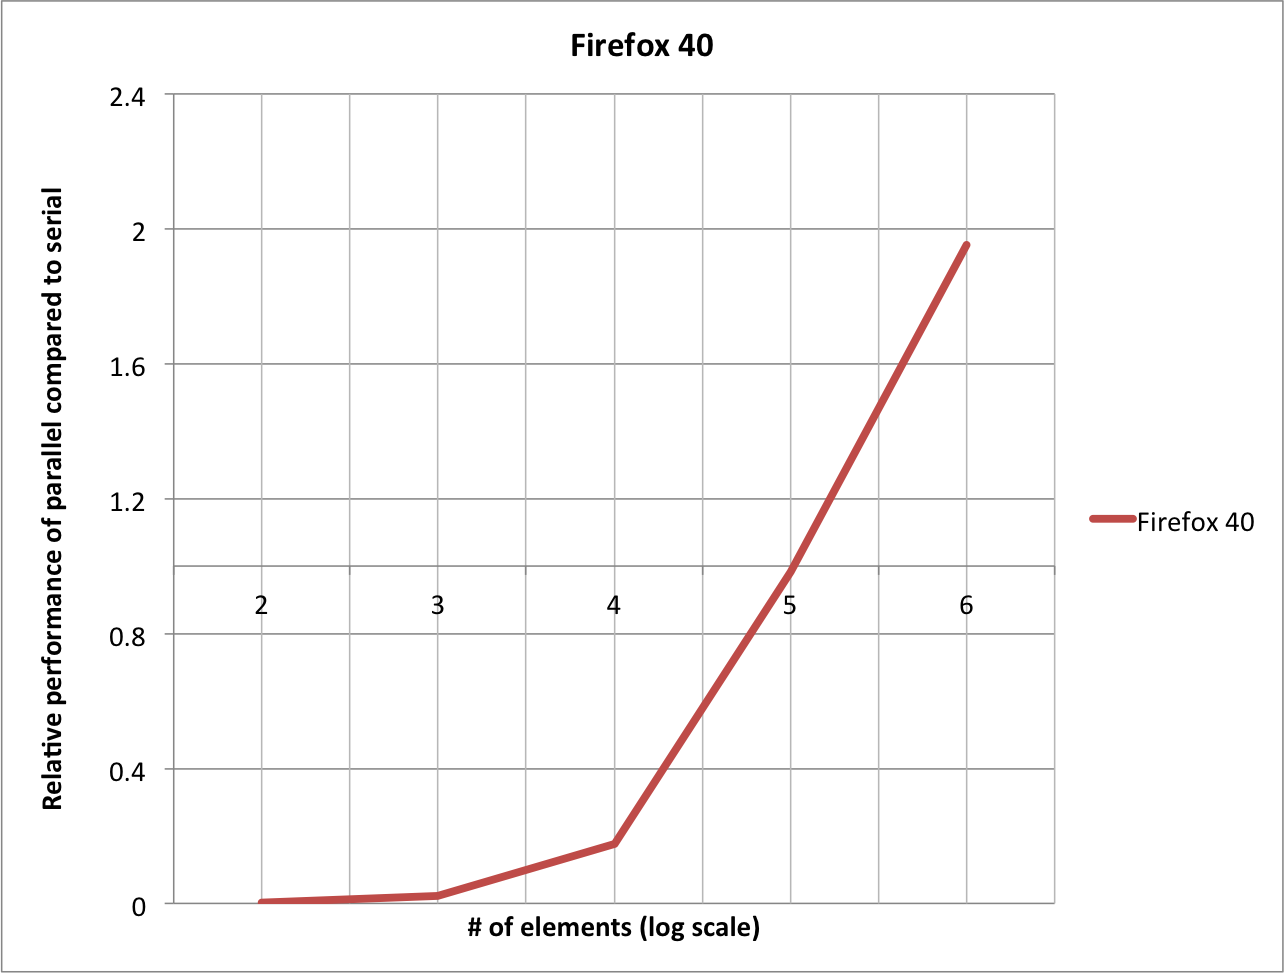
\includegraphics[height=7.7cm]{comparison}
\caption{Relative performance of parallel transformation compared to sequential one.}
\label{fig:relative}
\end{figure}

\subsection{Conclusion}
A couple of interesting findings result from the experiments. An expected one is that the amount of operations per second that can be performed with a serial implementation is almost inversely proportional to the amount of items to transform with a ratio of 1. On the other hand, this is not the case for the parallel approach.

An acceptable speedup of approximately \textbf{2.3x} can be achieved with a relatively large amount of items (\(10E6\)) and performing a computationally expensive computation (generating pseudo-random numbers). Larger speedups might be possible by applying optimizations to the library and there might also be some potential improvements for operations with \verb+SharedArrayBuffer+s as they are likely not fully optimized, being that they are only an experimental feature in Firefox Nightly.

\section{Future Work}\label{sec:future}
There are still some parts of the library that would benefit from optimizations. Of particular interest to us is to perform further profiling of the code executing in each Web Worker. As of today, using browser profiling tools for Web Workers is not as simple as doing so for the UI thread.\\

During our research we found that browser memory usage greatly increases when using shared memory after transforming an image multiple times. Memory is relased after a particular time period (which seems to indicate there is not a leak), but while memory usage is high, performance degrades. We plan to spend some time on this issue.\\

There is a strawman proposal to support typed objects \cite{typed-objects} in a future version of EcmaScript, which in turn would allow \verb+TypedArray+s of said typed objects. Once a browser has an experimental version available we intend to make sure that typed arrays of typed objects work with the library.\\

Once the \verb+SharedArrayBuffer+ type is available in other browsers (there is already a proposal for Google Chrome \cite{sab-chrome}) we plan to perform benchmarks and tests to compare with Firefox Nightly.

\subsubsection*{Acknowledgments.}
Thanks to Rosa Wachenchauzer, our tutor, for reviewing this paper and also for all her support and guidance throughout this entire project.

\begin{thebibliography}{4}

\bibitem{moore65} Moore, G.E.: Cramming More Components onto Integrated Circuits. (1965)

\bibitem{ms-par} Parallel Programming in the .NET Framework, Microsoft Corp., \url{http://msdn.microsoft.com/en-us/library/dd460693(v=vs.110).aspx}

\bibitem{es-web} EcmaScript, ECMA, \url{http://www.ecmascript.org/}

\bibitem{asm-web} asm.js, \url{http://asmjs.org/}

\bibitem{webgl-web} WebGL, Khronos Group, \url{http://www.khronos.org/webgl/}

\bibitem{rivertrail} Herhut, S., Hudson, R. L., Shpeisman, T., Sreeram, J.: River trail: A path to parallelism in javascript. SIGPLAN Not., 48(10):729--744, (2013).

\bibitem{par-js} Wang, J., Rubin, N., Yalamanchili, S.: River trail: ParallelJS: An Execution Framework for JavaScript on Heterogeneous Systems. SIGPLAN Not. (2014)

\bibitem{js-simd} McCutchan, J., Feng, H., Matsakis, N. D., Anderson, Z., Jensen, P.: A SIMD Programming Model for Dart, JavaScript, and other dynamically typed scripting languages (2014)

\bibitem{w3c-ww} Web Workers, W3C, \url{http://www.w3.org/TR/workers/}

\bibitem{event-loop} Concurrency model and Event Loop, Mozilla Developer Network, \url{https://developer.mozilla.org/en-US/docs/Web/JavaScript/EventLoop}

\bibitem{v8} v8, Google, \url{https://developers.google.com/v8/intro}

\bibitem{spider-monkey} SpiderMonkey, Mozilla, \url{https://developer.mozilla.org/en-US/docs/Mozilla/Projects/SpiderMonkey}

\bibitem{thread-pool} Schmidt, D. C., Vinoski, S.,: Comparing Alternative Programming Techniques for Multi-threaded CORBA Servers: Thread Pool (1996)

\bibitem{sab} JavaScript Shared Memory, Atomics, and Locks, \url{https://docs.google.com/document/d/1NDGA_gZJ7M7w1Bh8S0AoDyEqwDdRh4uSoTPSNn77PFk/edit}

\bibitem{es6-ta} TypedArray objects, ECMA, \url{https://people.mozilla.org/~jorendorff/es6-draft.html#sec-typedarray-objects}

\bibitem{pjs-api} p-j-s API, \url{https://github.com/pjsteam/pjs/blob/dev/README.md}

\bibitem{promise} Promise, MDN, \url{https://developer.mozilla.org/en-US/docs/Web/JavaScript/Reference/Global_Objects/Promise}

\bibitem{html-whatwg} HTML Standard, WHATWG, \url{https://html.spec.whatwg.org}

\bibitem{cloud-haskell} Epstein, J., Black, A. P., Peyton-Jones, S.: Towards Haskell in the Cloud (2011)

\bibitem{distributed-scheme} Schwendner, A.: Distributed Functional Programming in Scheme (2010)

\bibitem{encoding-api} Encoding Standard, WHATWG, \url{https://encoding.spec.whatwg.org}

\bibitem{benchmark} Sepia tone transformation benchmark comparison between p-j-s and plain JS, \url{http://jsperf.com/pjs-map-vs-serial/9}

\bibitem{typed-objects} Typed Objects, ECMA, \url{http://wiki.ecmascript.org/doku.php?id=harmony:typed_objects}

\bibitem{sab-chrome} Shared Array Buffers, Chromium Dashboard, \url{https://www.chromestatus.com/feature/4570991992766464}

\end{thebibliography}

\end{document}
